% ~~~ [ Native Code to LLVM IR ] ~~~~~~~~~~~~~~~~~~~~~~~~~~~~~~~~~~~~~~~~~~~~~~~

\subsubsection{Native Code to LLVM IR}
\label{sec:design_native_code_to_llvm_ir}

%    - binary -> LLVM IR ([MC-Semantics](https://github.com/trailofbits/mcsema), [Dagger](http://dagger.repzret.org/) or [Fracture](https://github.com/draperlaboratory/fracture))

There exist several open source projects which translate

\ref{fig:front-end_binary}

\begin{figure}[htbp]
	\begin{center}
		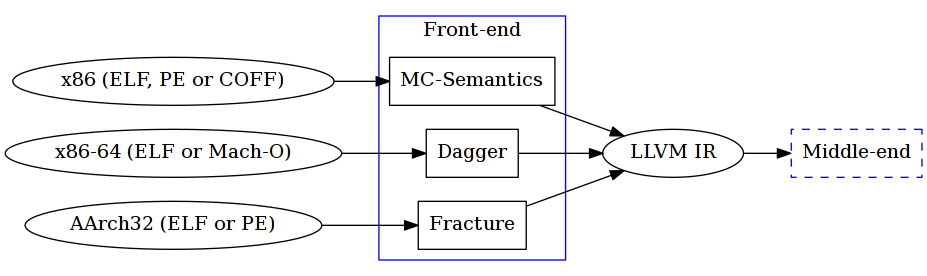
\includegraphics[width=\textwidth]{inc/front-end_binary.png}
		\caption{The three open source projects MC-Semantics, Dagger and Fracture translate native code of various architectures (e.g. x86, x86-64 and ARM) and file formats (e.g. ELF, PE, COFF and Mach-o) to LLVM IR.}
		\label{fig:front-end_binary}
	\end{center}
\end{figure}
